\documentclass[aip,rsi,amsmath,amssymb,reprint, english]{revtex4-1}

\usepackage[utf8]{inputenc}
\usepackage{amsmath}
\usepackage{amsfonts}
\usepackage{amssymb}
\usepackage{amsthm}
\usepackage{physics}
\usepackage{graphicx}
\usepackage{booktabs}
\usepackage{xcolor}
\usepackage[colorlinks=true,linkcolor=blue,urlcolor=blue,citecolor=blue]{hyperref}

\graphicspath{ {images/} }

\setlength\parindent{0pt}


\begin{document}
	
\title{Notes on: Two holes $S-T_-$ transition by controlling detuning in the presence of SOC}
\author{David Fernández Fernández}
\email[]{david.fernandezf03@estudiante.uam.es}
\date{\today}

\maketitle

\section{Model} \label{sec:Model}
The two holes confined in a double quantum dot (DQD) in the presence of a external magnetic field perpendicular to the dots and in absence of spin-orbit coupling (SOC) can be written in the second quantization Hamiltonian as

\begin{equation}
	H=\sum_{i\sigma}\varepsilon_{i\sigma}n_{i\sigma}+u\sum_in_{i\uparrow}n_{i\downarrow}-\tau\sum_{\sigma}\left(c_{1\sigma}^{\dagger}c_{2\sigma}+H.c.\right)
\end{equation}

where $\varepsilon_{i\sigma}$ represent the energy of the single-particle located in the dot $i=1,2$ with spin $\sigma=\uparrow,\downarrow=\pm1/2$, this energy counts the bias energy level of the dot and the Zeeman splitting $\varepsilon_{i\sigma}=\varepsilon_{i}+g\mu_BB\sigma$, $g=1.35$ for GaAs. The intradot Coulomb interaction $u$ exist when various particles occupy the same dot. There is also a spin-conserving tunnelling term $\tau$ between the dots. The operators $c_{i\sigma}$ ($c^{\dagger}_{i\sigma}$) is the annihilating (creation) of a hole in the dot $j$ with spin $\sigma$. The energy spectrum for this model is given in the following figure: 

\begin{figure}[h!]
	\centering
	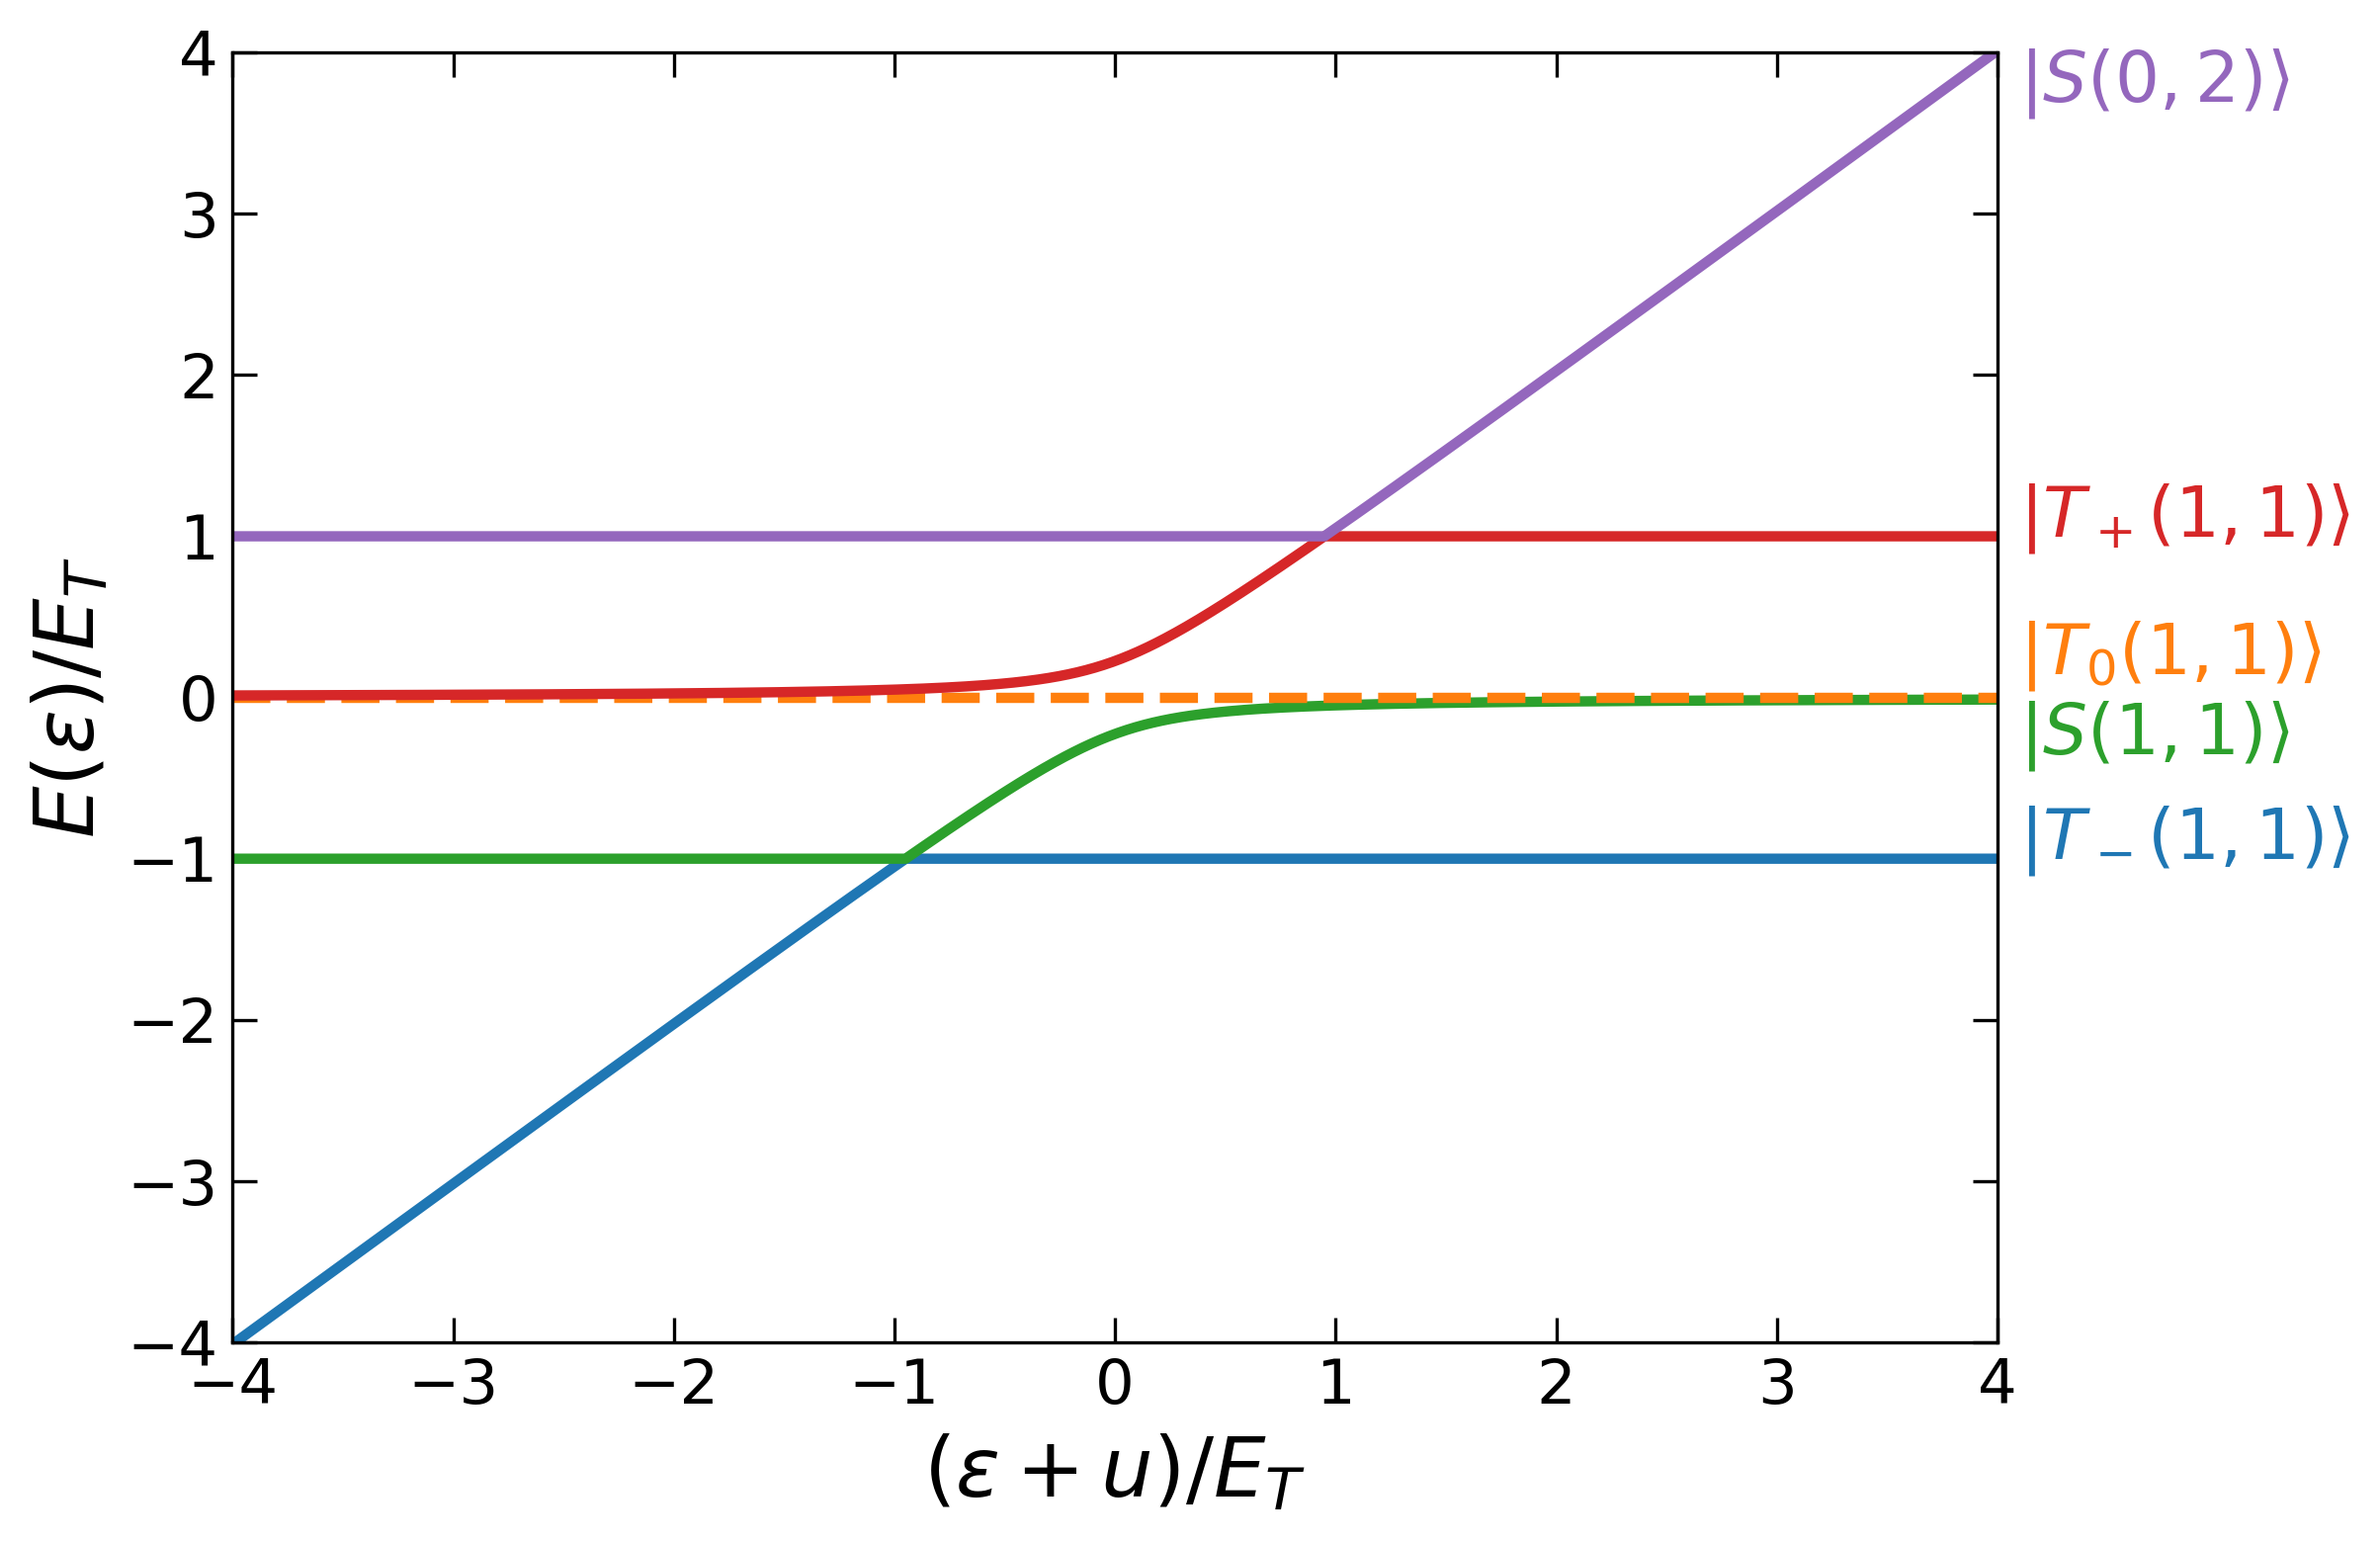
\includegraphics[width=\linewidth]{spectrum_5_levels_woSOC}
	\caption{Energy spectrum for two heavy holes confined in a DQD in absence of SOC. The parameters used are $u=3\; meV$, $\tau=0.25 \; \mu eV$, $B=20\; mT$ and $E_T=g\mu_B B=1.56 \; \mu eV$.}
	\label{fig:spectrum_1}
\end{figure}

where we have normalized the energies to the energy of the triplets $E_T=g\mu_BB$. To obtain this spectrum have excluded singlet state of double occupation in the left dot. It is usually to work with a antisymmetric bias gate for each dot $\varepsilon_R=-\varepsilon_L$, defining the difference as $\varepsilon\equiv\varepsilon_R-\varepsilon_L=2\varepsilon_R$. We can see in Fig. \ref{fig:spectrum_1} that the state $\ket{T_0(1,1)}$ does not interact with any other state. We are interested in the levels near the cross between the singlet states and $\ket{T_-(1,1)}$, that is in the neighbourhood of $(\varepsilon+u)/E_T=-1$. At this value of the detuning the other triplet state $\ket{T_+(1,1)}$ is too far away in energies, so can neglect it for the moment. We are left with a three level system, whose Hamiltonian is written as

\begin{equation}
	H=\bordermatrix{~ & \ket{T_-(1,1)} & \ket{S(1,1)} & \ket{S(0,2)}\cr
		~ & -E_T & 0 & 0 \cr
		~ & 0 & 0 & \sqrt{2}\tau \cr
		~ & 0 & \sqrt{2}\tau & \varepsilon+u \cr}
\end{equation}

The eigenenergies of this system are

 \begin{equation}
 	\begin{split}
 	E_S&=(u+\varepsilon-\sqrt{8\tau^2+(u+\varepsilon)^2})/2\\
 	E_{S^{\prime}}&=(u+\varepsilon+\sqrt{8\tau^2+(u+\varepsilon)^2})/2\\
 	E_{T_-}&=-E_T
 	\end{split}
 \end{equation}
 
 corresponding to two hybridized singlets and one triplet with eigenvectors
 
 \begin{equation}
 	\begin{split}
 	\ket{S}&=c(\varepsilon)\ket{S(1,1)}+\sqrt{1-c(\varepsilon)^2}\ket{S(0,2)}\\
 	\ket{S^{\prime}}&=c^{\prime}(\varepsilon)\ket{S(1,1)}+\sqrt{1-c^{\prime}(\varepsilon)^2}\ket{S(0,2)}\\
 	\ket{T}&=\ket{T_-}
 	\end{split}
 	\label{eq:hibrid_coefficients}
 \end{equation}

where $c(\varepsilon)$ and $c^{\prime}(\varepsilon)$ are some functions whose explicit formula is not relevant at all. What is really import is the dependence of this coefficients with the detuning, what can be observed in Fig. \ref{fig:coefficients}.

\begin{figure}[h!]
	\centering
	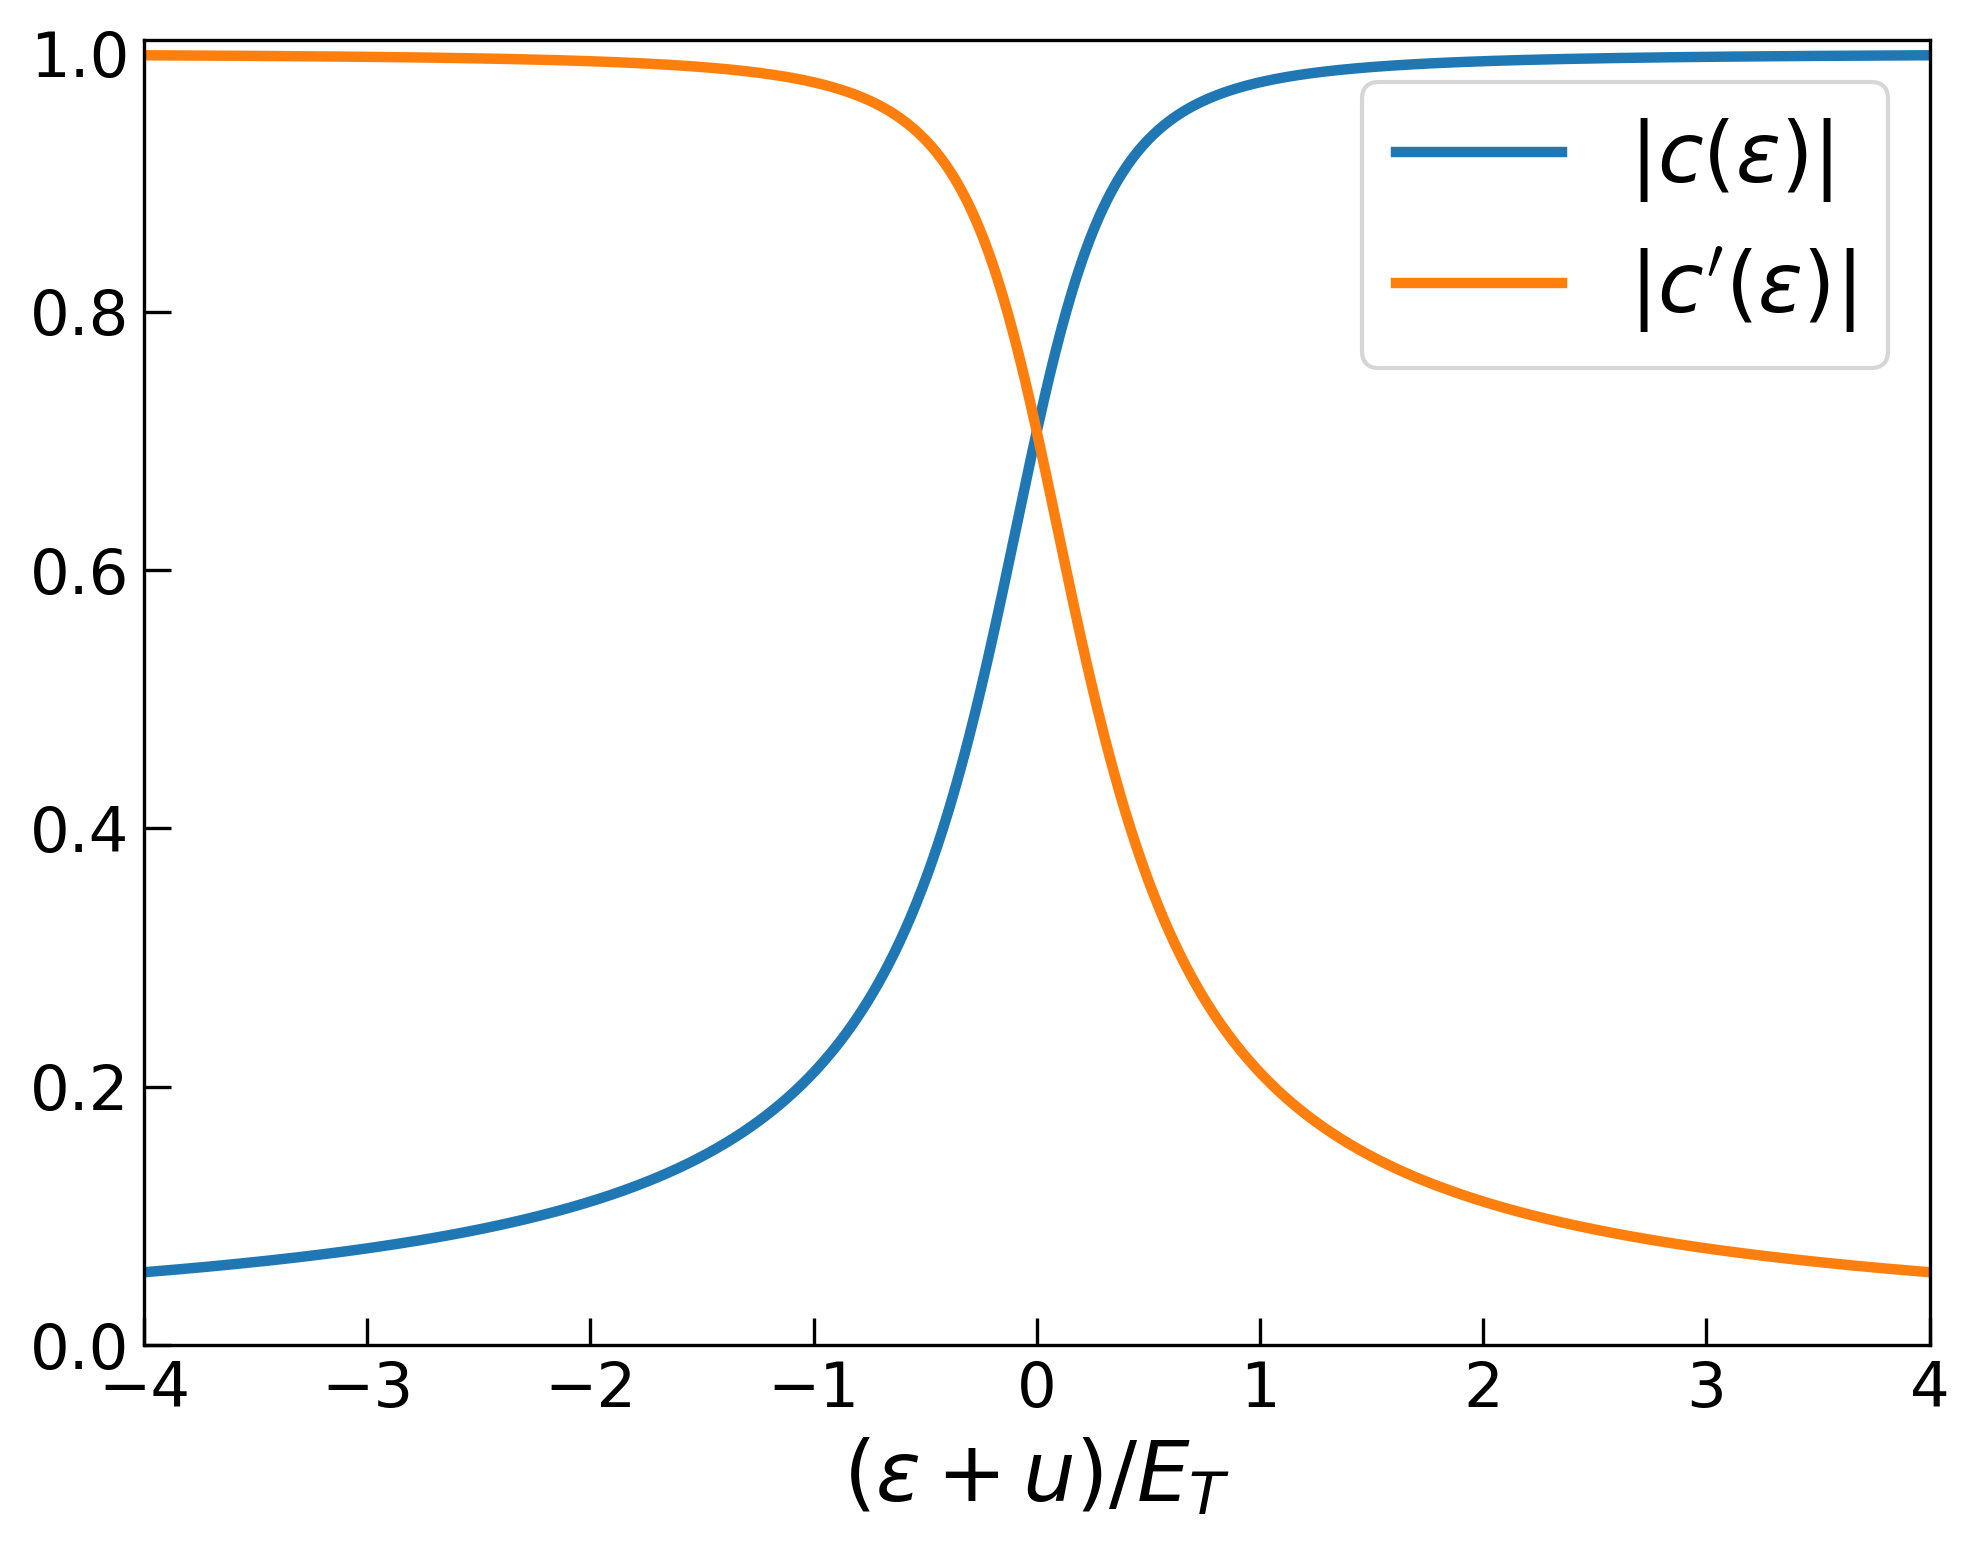
\includegraphics[width=.8\linewidth]{coefficients}
	\caption{Dependence of $c(\varepsilon)$ and $c^{\prime}(\varepsilon)$ with the detuning. The parameters used are the same as those given in Fig. \ref{fig:spectrum_1}.}
	\label{fig:coefficients}
\end{figure}

If we consider spin-orbit coupling we have to introduce two different terms, the Dresselhaus SOC $H_D=\beta(\sigma_+p_-p_+p_--\sigma_-p_+p_-p_+)$ and the Rashba SOC $H_R=i\alpha E_{\perp}(\sigma_+p_-^3-\sigma_-p_+^3)$. Since this terms couple states with different total spin, SOC gives rise the terms $\lambda_1=\bra{T_-(1,1)}H_D+H_R\ket{S(1,1)}$ and $\bra{T_-(1,1)}H_D+H_R\ket{S(0,2)}$. For simplicity we take both SOC parameters to be equal $\alpha E_{\perp}=\beta$. To obtain some analytical expression for this coupling terms we suppose the single hole orbital function as Gaussian waves centred in each dot $\psi_i=\dfrac{1}{l}\sqrt{\dfrac{2}{\pi}}\exp(-\dfrac{(x-x_i)^2+y^2}{l^2})$, where the dots lies in the $x$ axis, $d$ is the interdot distance, $x_1=-x_2=d/2$, and $l$ is the extent of the wave function. After integrating, the coupling terms are $\lambda_1=\dfrac{8\alpha E_{\perp}d}{l^4}\exp(-d^2/l^2)$ and $\lambda_2=\dfrac{4\sqrt{2}\alpha E_{\perp}d}{l^4}\exp(-d^2/2l^2)$. In the base of the triplet state and the two hybridized the Hamiltonian including the SOC is written as

\begin{equation}
	H=\bordermatrix{~ & \ket{T_-(1,1)} & \ket{S} & \ket{S^{\prime}}\cr
		~ & -E_T & \lambda & \lambda^{\prime} \cr
		~ & \lambda & E_S & 0 \cr
		~ & \lambda^{\prime} & 0 & E_{S^{\prime}} \cr}
\end{equation}

where $\lambda=c(\varepsilon)\lambda_1+\sqrt{1-c(\varepsilon)^2}\lambda_2$ and $\lambda^{\prime}=c^{\prime}(\varepsilon)\lambda_1+\sqrt{1-c^{\prime}(\varepsilon)^2}\lambda_2$. If we choose $l=d/2$ we can obtain $\lambda_1/\lambda_2=1/100$ and then $\lambda\approx \sqrt{1-c(\varepsilon)^2}\lambda_2$. The energy spectrum of this three level system, now with SOC is shown in Fig. \ref{fig:spectrum_2}.

\begin{figure}[h!]
	\centering
	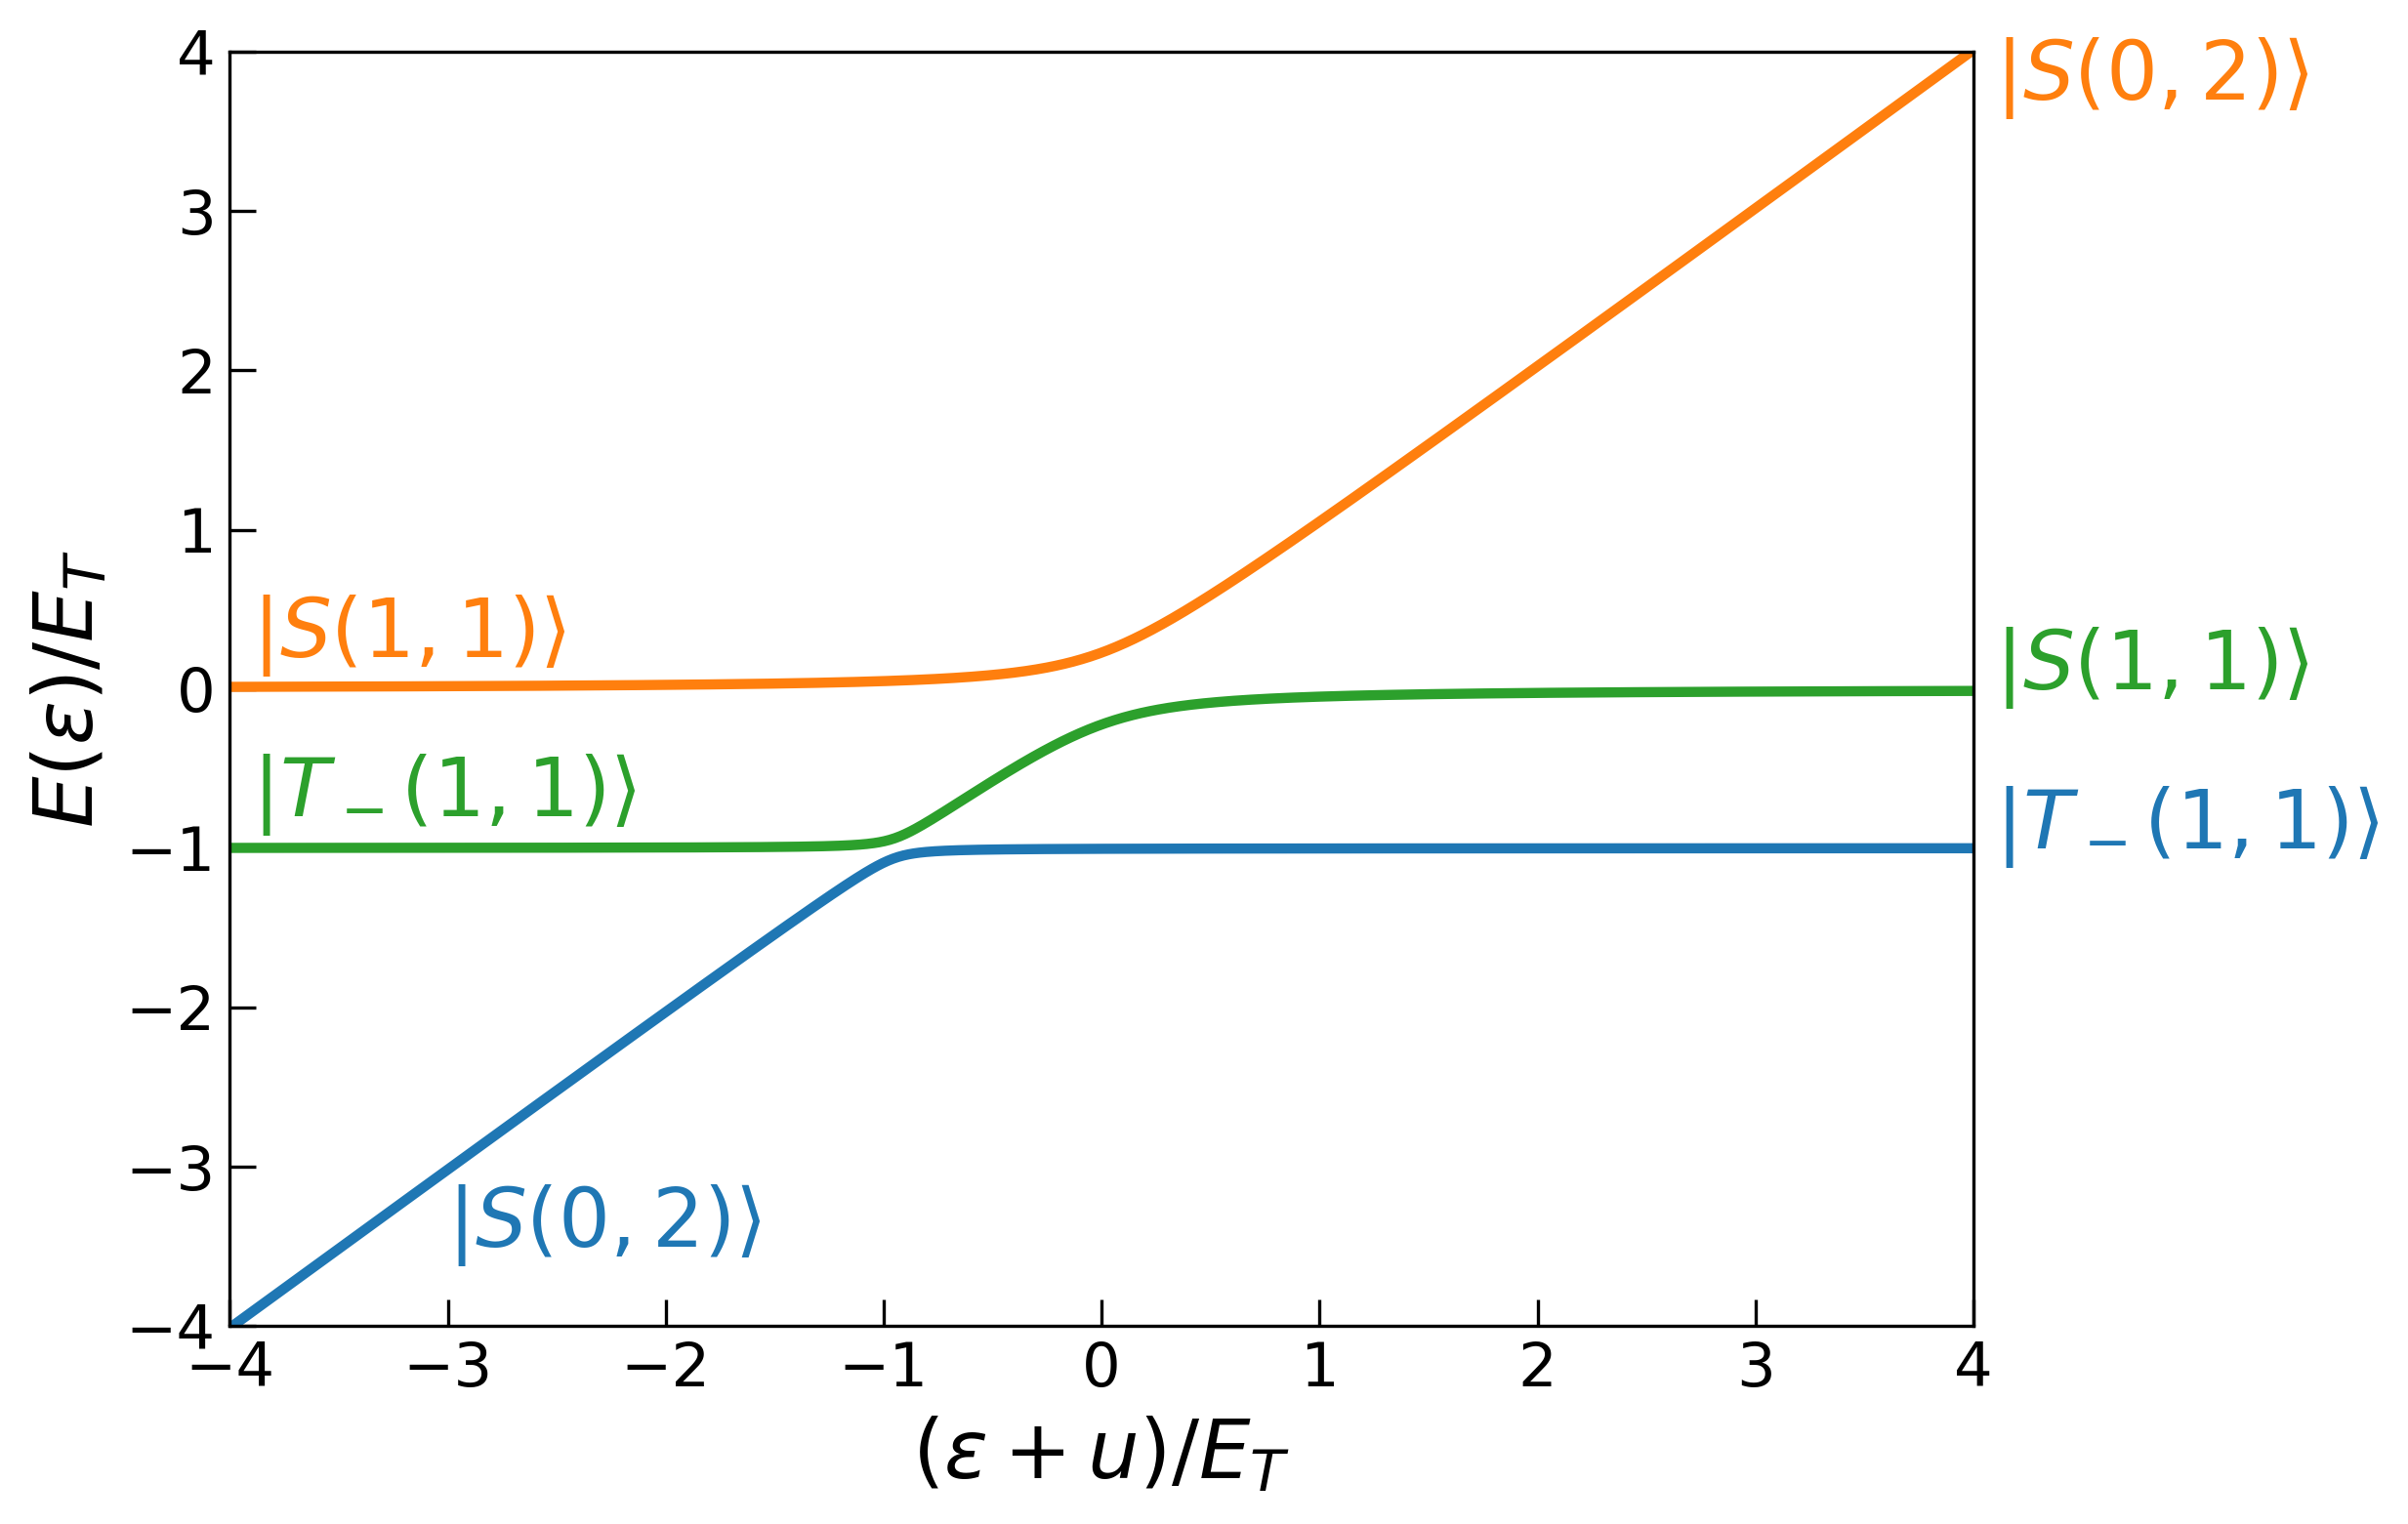
\includegraphics[width=\linewidth]{spectrum_3_levels_wSOC}
	\caption{Energy spectrum for two heavy holes confined in a DQD in presence of SOC. The parameters used are $u=3\; meV$, $\tau=0.25 \; \mu eV$, $\lambda_1=0.001 \mu eV$, $\lambda_2=0.1\mu eV$, $B=20\; mT$ and $E_T=g\mu_B B=1.56 \; \mu eV$.}
	\label{fig:spectrum_2}
\end{figure}

To simplify even more the problem we can deal with the subspace conformed by the lowest energy hybridized singlet and the triplet. The effective Hamiltonian, after shifting the energies by $(E_T-E_S)/2$, is 

\begin{equation}
	H_{\text{eff}}(\varepsilon)=\mqty(\Delta(t) & \lambda \\ \lambda & -\Delta (t))
\end{equation} 

where $\Delta\equiv-(E_S+E_T)/2$.

\section{Fast Quasiadiabatic Approach (FAQUAD)}

We want to perform the transfer from $\ket{1}=\ket{T_-(1,1)}$ to $\ket{2}=\ket{S}$ as quickly as possible at all times. To obtain that we use the fast quasiadiabatic approach that engineers the time dependence function $\Delta(t)$ (at this moment we will neglect the dependence on the detuning on the parameter $\lambda$ \textcolor{red}{(THIS IT NOT CORRECT AT ALL)}. The standard adiabatic parameter is imposed to be constant, and is given by

\begin{equation}
	\hbar\abs{\dfrac{\braket{\phi_1(t)}{\partial_t\phi_2(t)}}{E_1(t)-E_2(t)}}=c
\end{equation}

Since we are interested in the dependence of $\Delta(t)$, we can apply the chain rule to obtain the differential equation

\begin{equation}
	\dfrac{d \Delta}{ds}=\dfrac{\tilde{c}}{\hbar}\abs{\dfrac{E_1-E_2}{\braket{\phi_1}{\partial_{\Delta}\phi_2}}}
	\label{eq:EDO_Delta}
\end{equation}

where we have defined $s\equiv t/t_F$ and 

\begin{equation}
	\tilde{c}\equiv ct_F=\hbar\int^{\Delta(t_F)}_{\Delta(0)}\dfrac{d\Delta}{\abs{\dfrac{E_1-E_2}{\braket{\phi_1}{\partial_{\Delta}\phi_2}}}}
\end{equation}

In our particular case, the two eigenvectors of the Hamiltonian $H_{\text{eff}}$ are

\begin{equation}
	\begin{array}{cc}
	\ket{\phi_1}=\mqty(\cos\theta/2 \\ \sin \theta/2) & \ket{\phi_2}=\mqty(\sin\theta/2 \\ -\cos\theta/2)
	\end{array}
\end{equation}

where $\tan\theta/2=[-\Delta+\sqrt{\Delta^2+\lambda^2}]/\lambda$, and $E_1-E_2=2\sqrt{\Delta^2+\lambda^2}$. After some algebra we obtain

\begin{equation}
	\abs{\dfrac{E_1-E_2}{\braket{\phi_1}{\partial_{\Delta}\phi_2}}}=\dfrac{4(\Delta^2+\lambda^2)^{1.5}}{\lambda}
\end{equation}

We will go from $(\varepsilon(0)+u)/E_T=-4$ to $(\varepsilon(t_F)+u)/E_T=4$, after numerical integration we obtain a value of $\tilde{c}=3.26 \; ns$. The typical final times are $t_F\sim 10 \; ns$ giving an adiabatic parameter of $c\sim 0.3<1$. Once obtained the value for this constant we can solve numerically the differential equation (Eq. \ref{eq:EDO_Delta}) to obtain the dependence of $\Delta$ with time (or with the variable $s$).

The next step is to solve the dynamics of the system, for what we will use the density matrix, solving numerically the EDO given by

\begin{equation}
	\dfrac{d \rho(t)}{d t}=-\dfrac{i}{\hbar}\comm{H_{\text{eff}}(t)}{\rho(t)}
\end{equation}

\section{Results}

The result obtained for the variation of the detuning in terms of the time is represented in Fig. \ref{fig:detuning_1}.

\begin{figure}[h!]
	\centering
	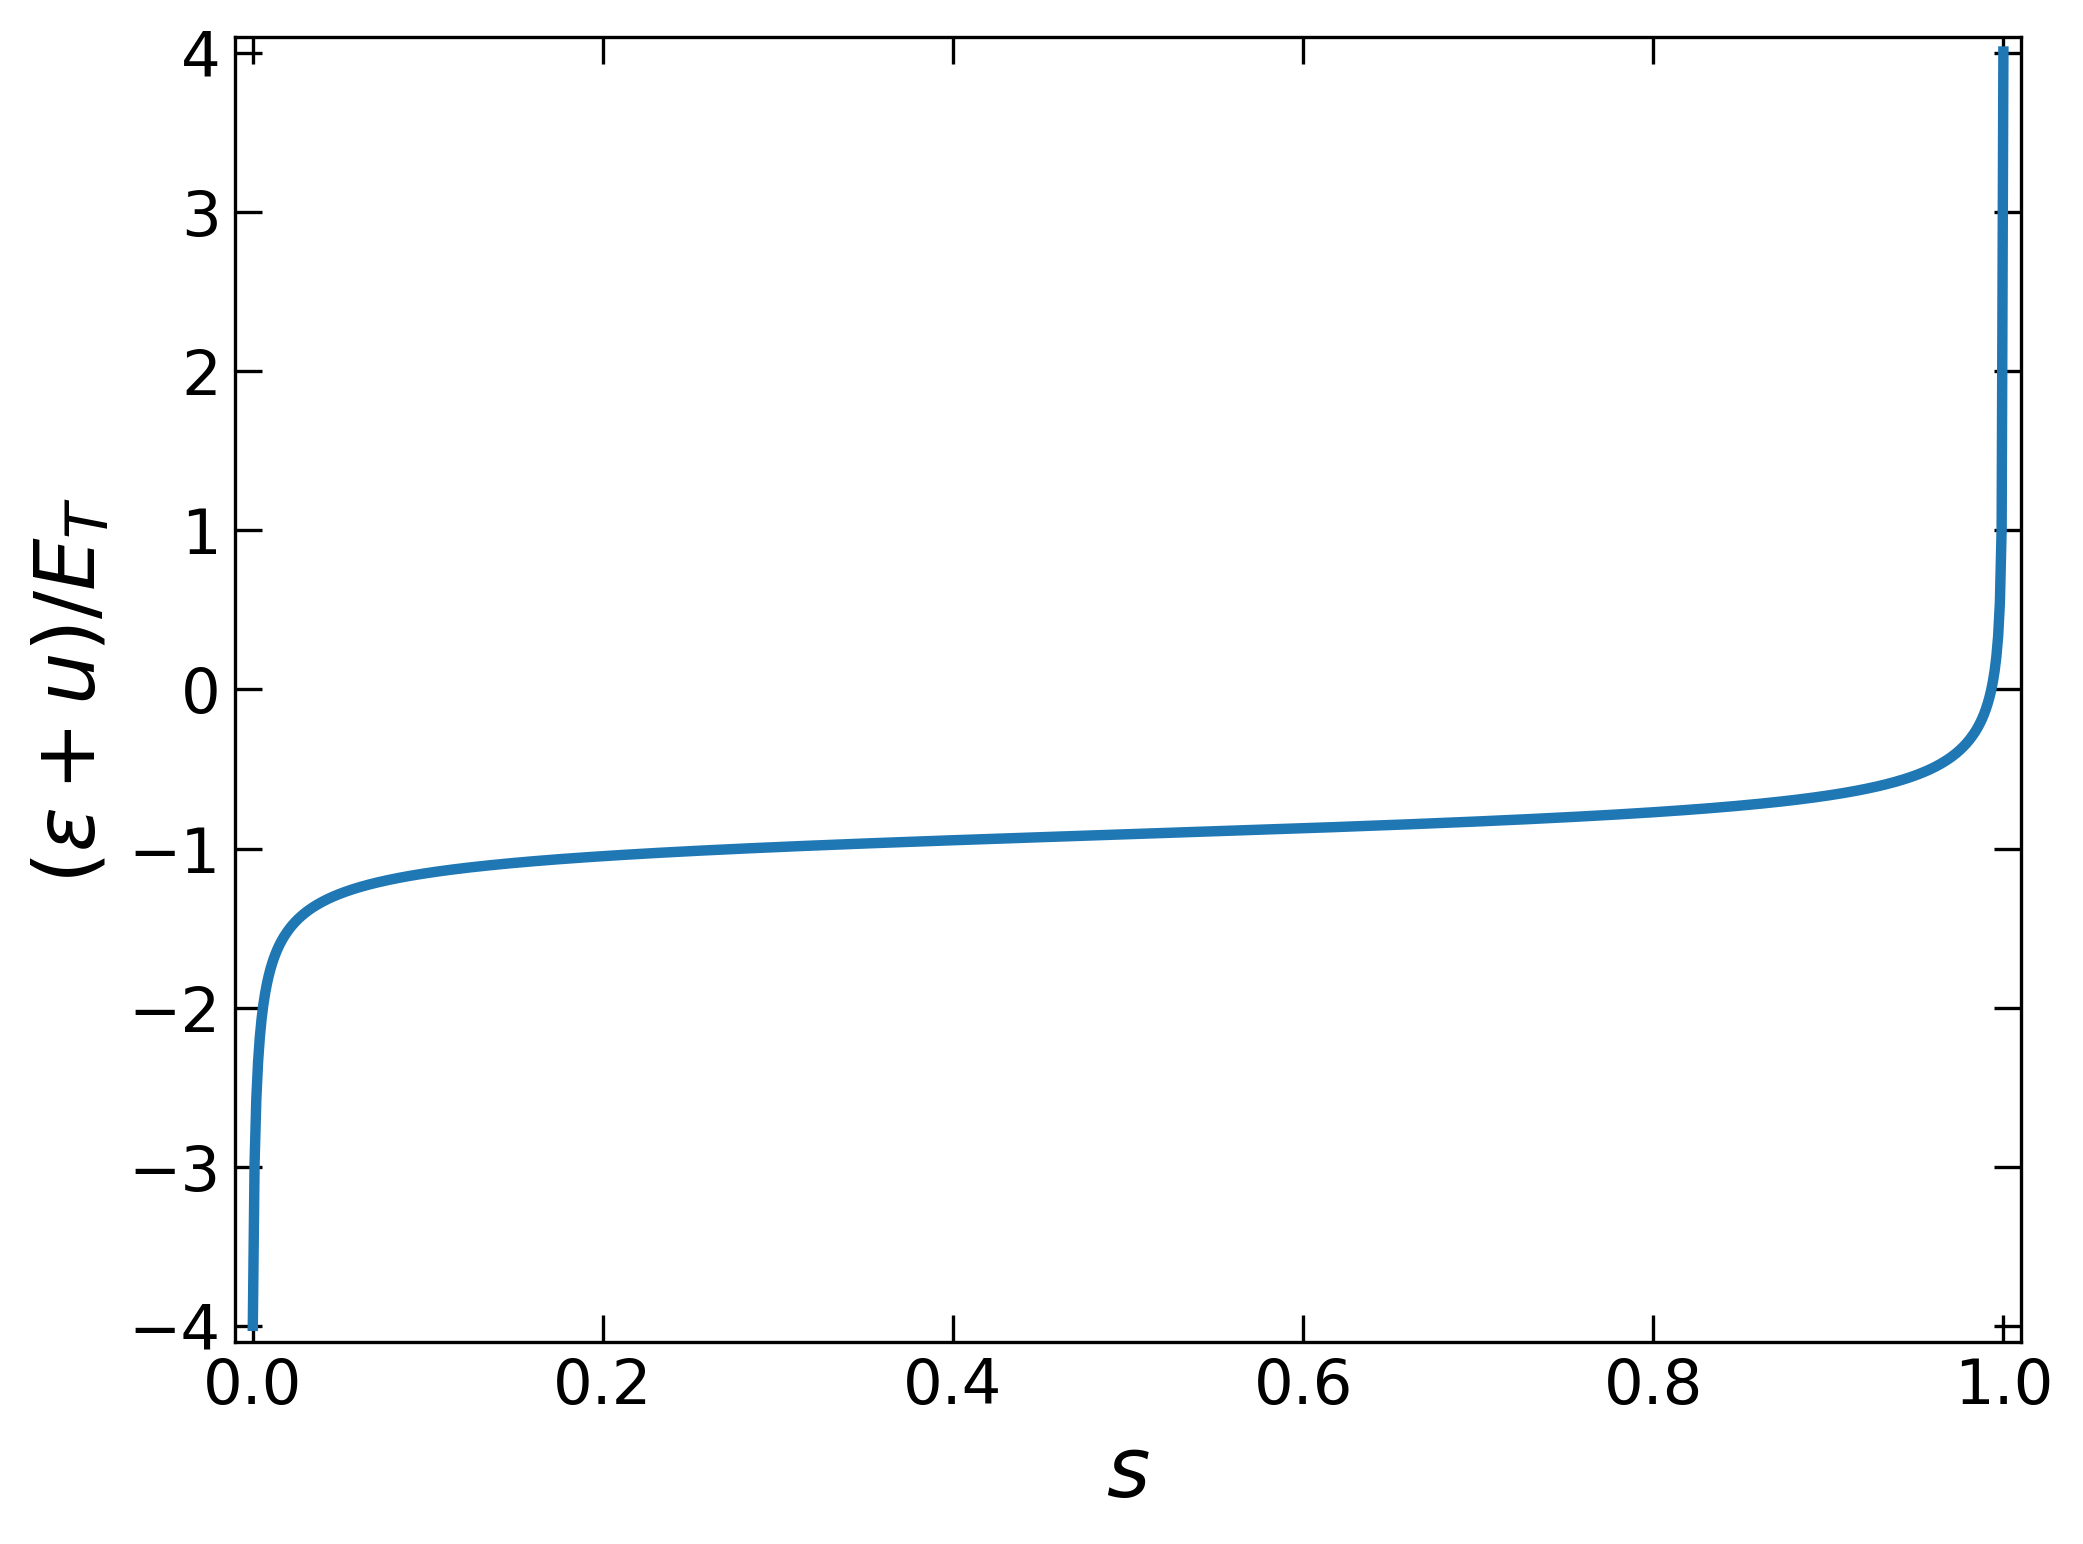
\includegraphics[width=\linewidth]{detuning_1}
	\caption{Detuning in terms of $s\equiv t/t_F$.}
	\label{fig:detuning_1}
\end{figure}

In the next figure is represented the fidelity of the protocol defined as the occupation of the hybrid singlet state at the end of the procedure.

\begin{figure}[h!]
	\centering
	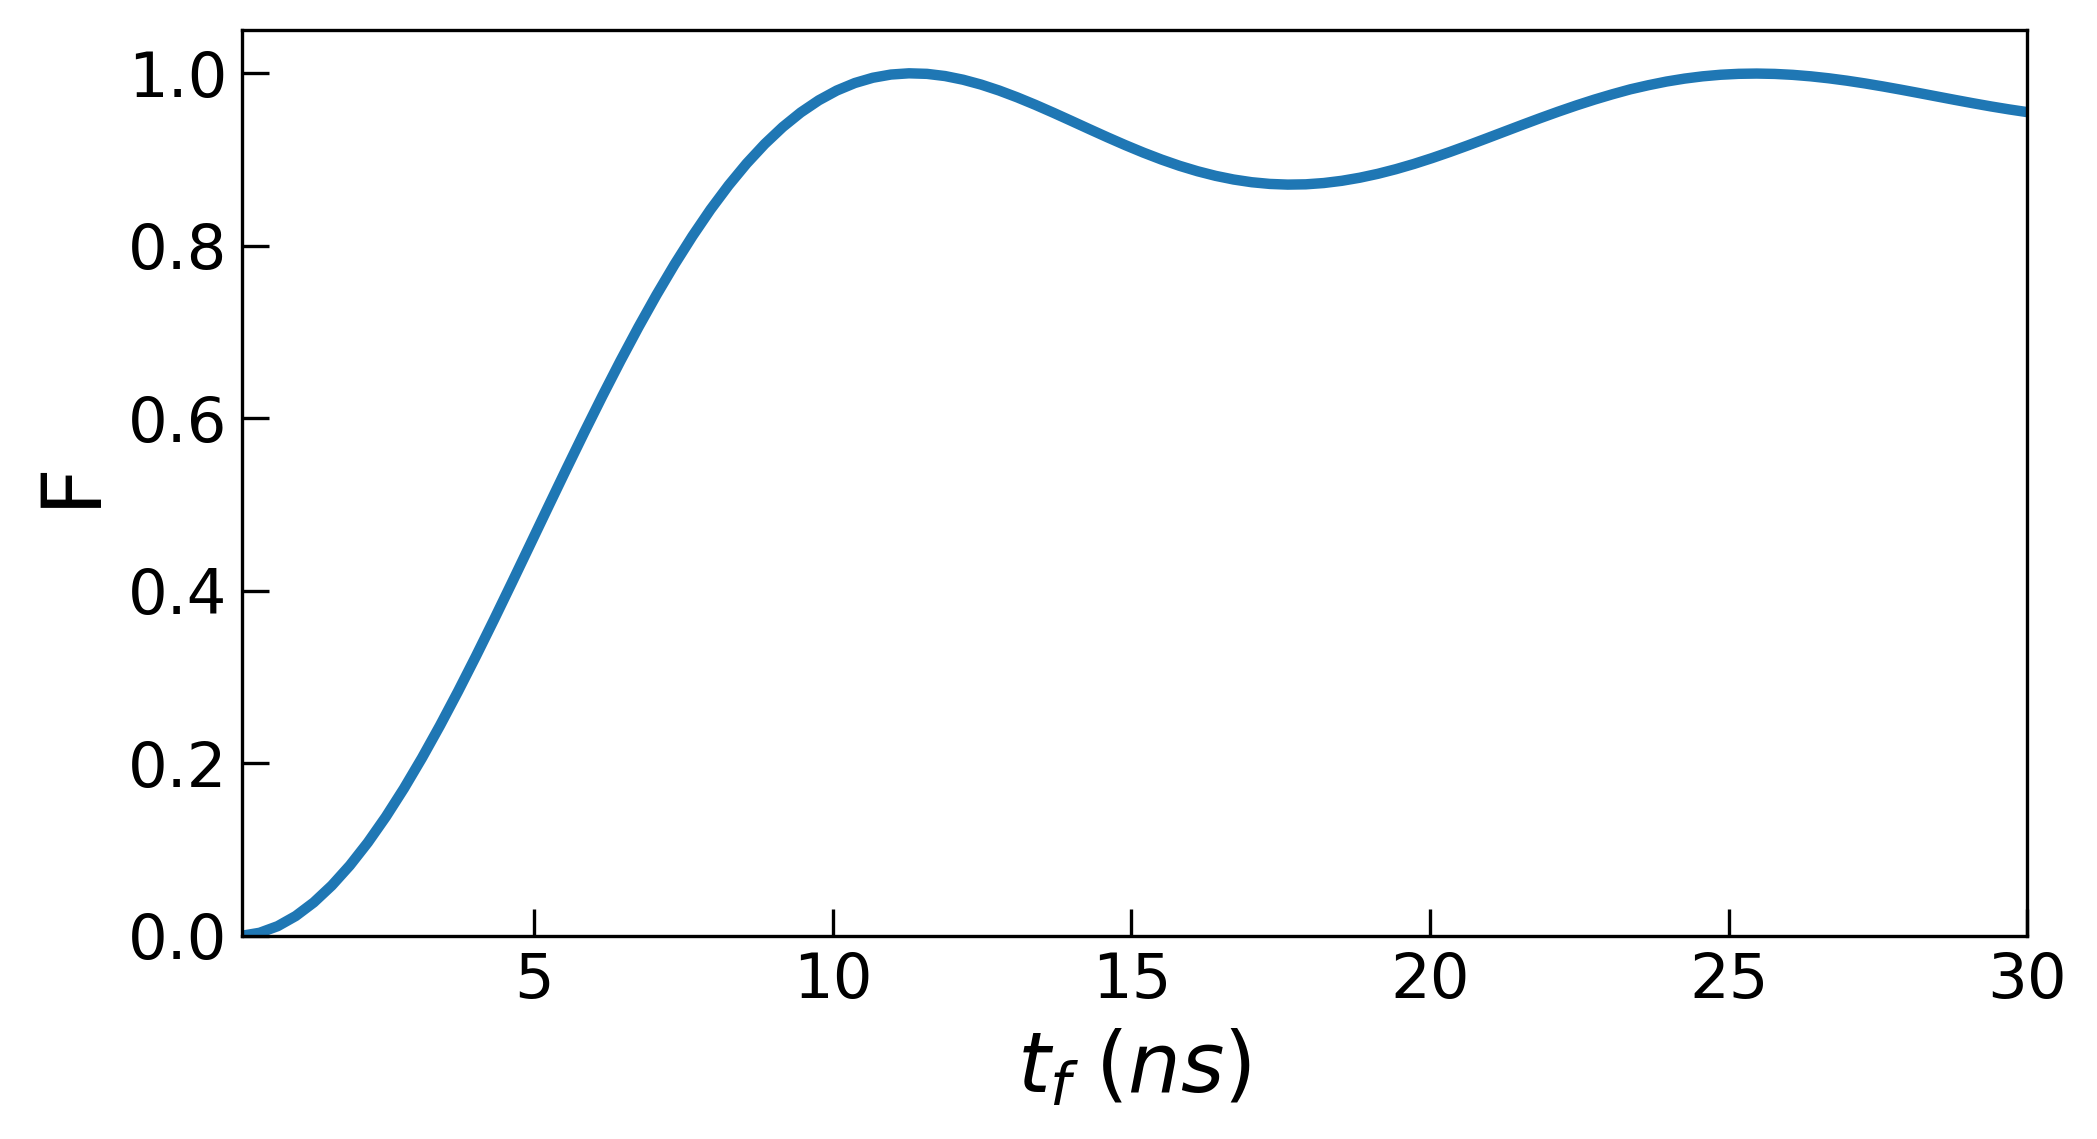
\includegraphics[width=\linewidth]{fidelity_1}
	\caption{Fidelity of the procedure for different final times. The fidelity is defined as $F\equiv \abs{\braket{S}{\psi(t_F)}}^2$.}
	\label{fig:fidelity_1}
\end{figure}

The first maximum obtained for the fidelity correspond to $99.97\% $ reached at the final time $t_F=11.17 \; ns$. But we are not only interested in going from the triplet to the singlet state, but we also need to populate the double occupation state as little as possible. Using the coefficients given in Eq. (\ref{eq:hibrid_coefficients}) we can see the population for each of the three states

\begin{figure}[h!]
	\centering
	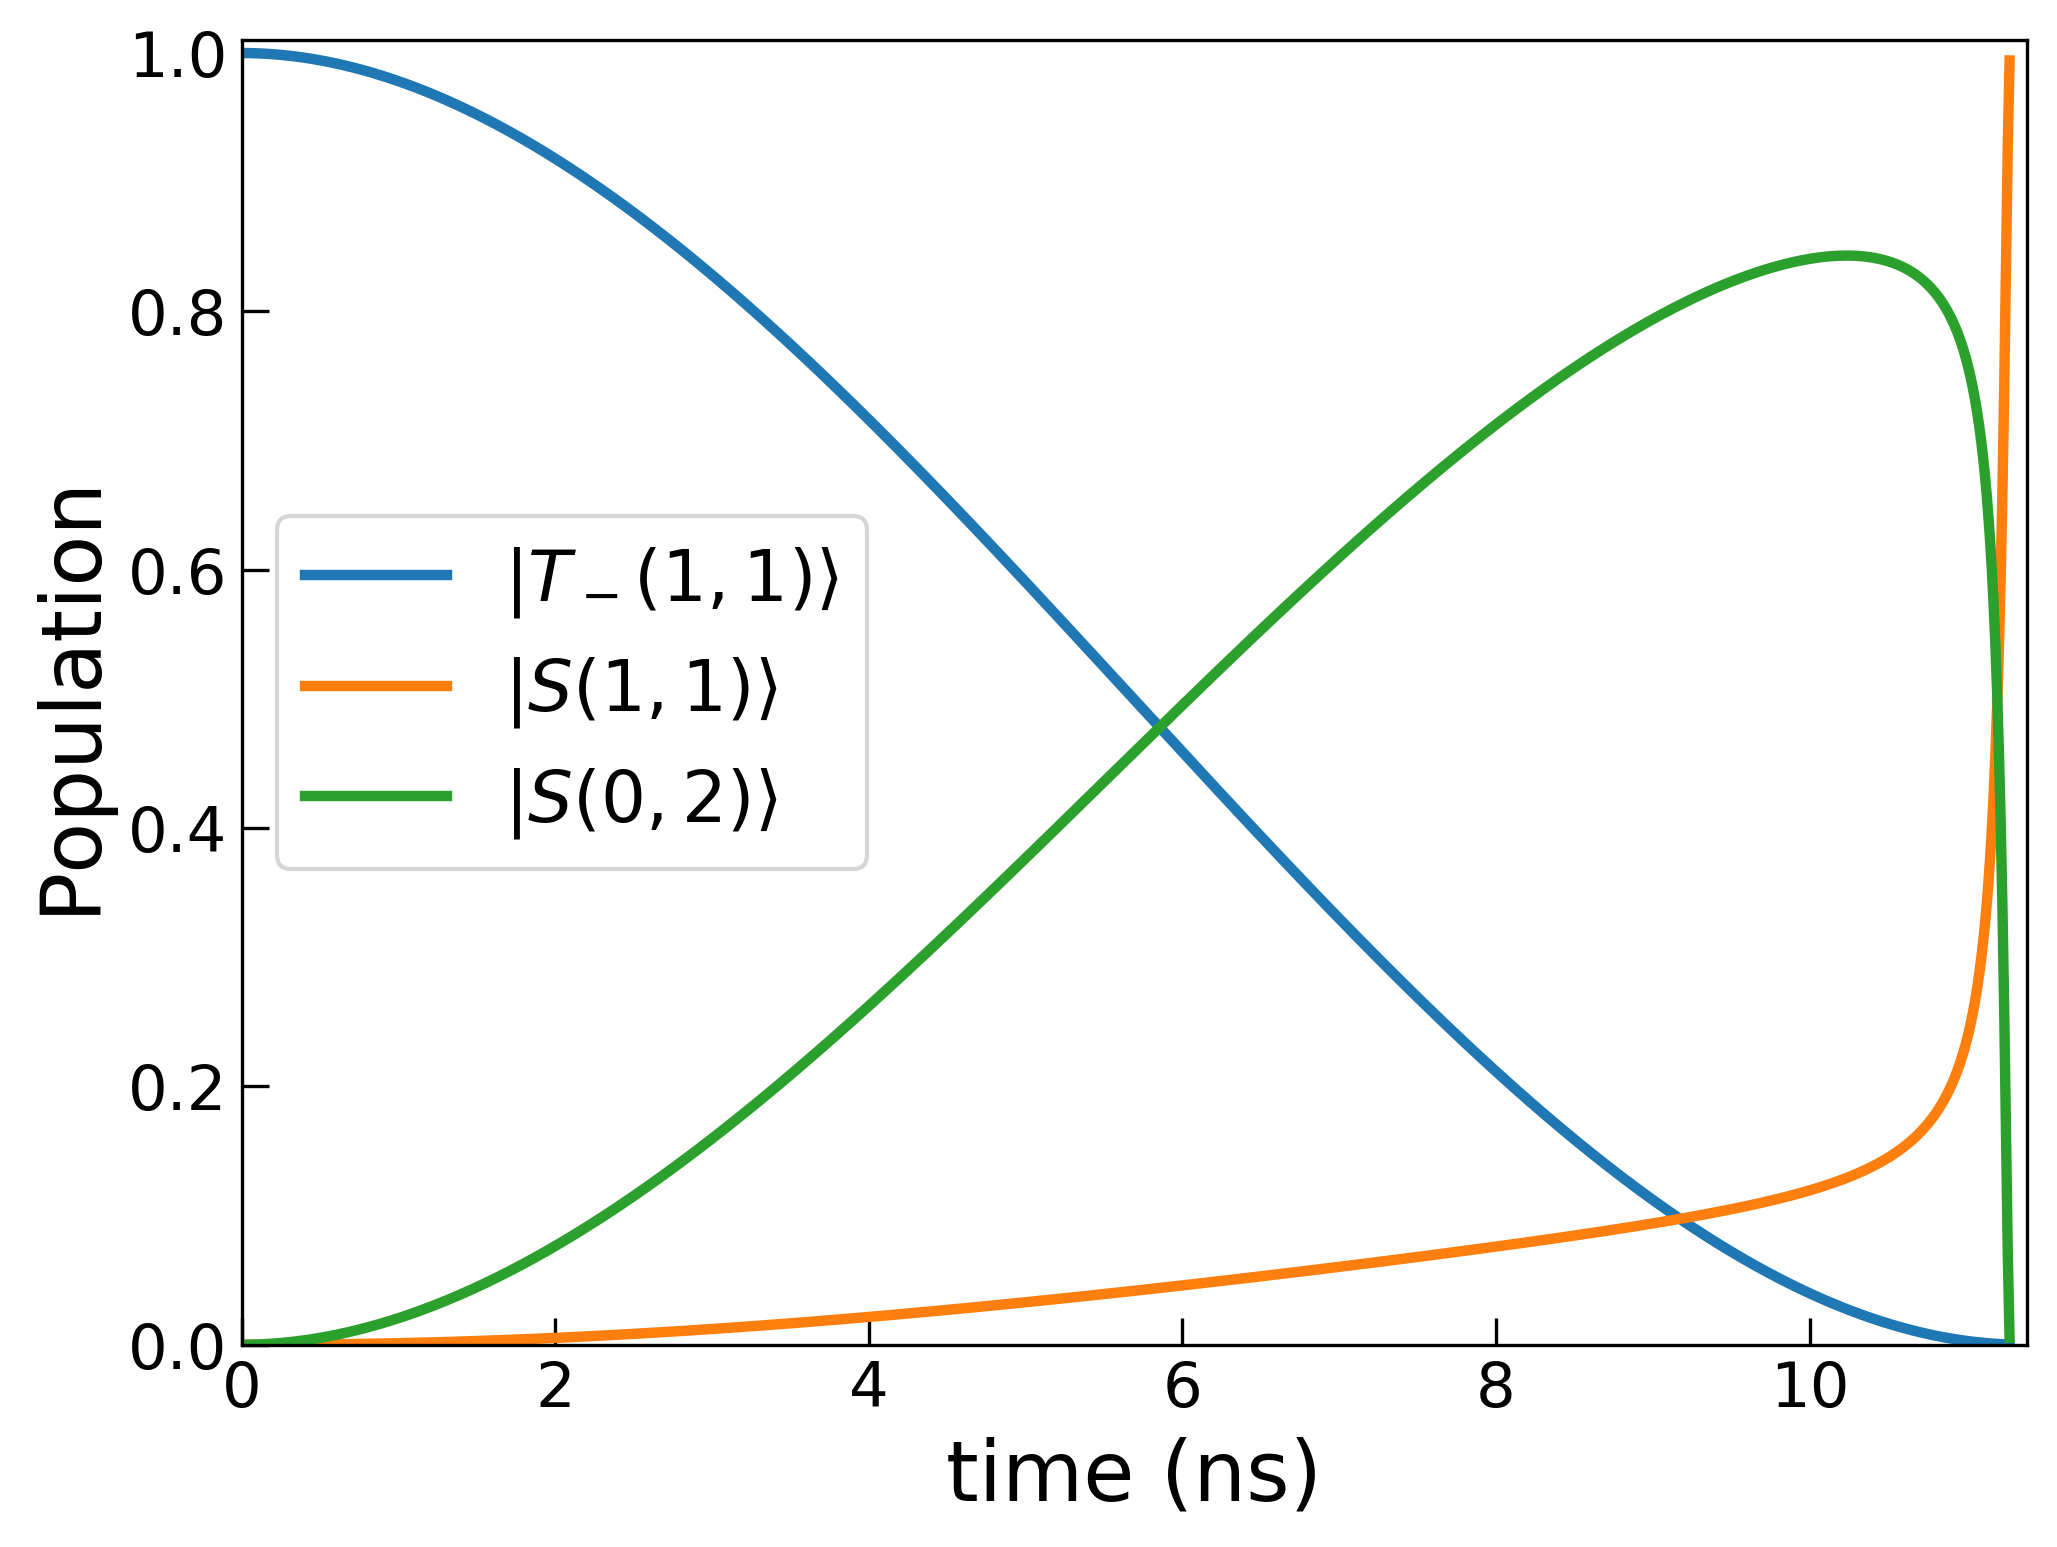
\includegraphics[width=\linewidth]{population_1}
	\caption{Population of the different states (two singlets and one triplet) for the case of $t_F=11.17 \, ns$.}
	\label{fig:population_1}
\end{figure}

We can see that at the end of the procedure we populate almost completely the single occupation singlet, but the population of $\ket{S(0,2)}$ is too high during the protocol.

\section*{TO DO LIST}

\begin{itemize}
	
	\item Introduce the dependence of $\lambda(\varepsilon)$, we can see in Fig. \ref{fig:coefficients} that $c(\varepsilon)$ is not constant in the range of detuning that we use.
	
	\item Interpolate $\Delta(\varepsilon)$ since in the final times the density of points is too poor, giving as consequence the abrupt change of the population in Fig. \ref{fig:population_1}.
	
	\item Include the state $\ket{S^{\prime}}$ since we can see in Fig. \ref{fig:spectrum_2} that at $(\varepsilon+u)/E_T=0$ the two hybrid singlets are too near in energies to be neglected.
\end{itemize}

	
\end{document}